\begin{figure}
	\centering
	
	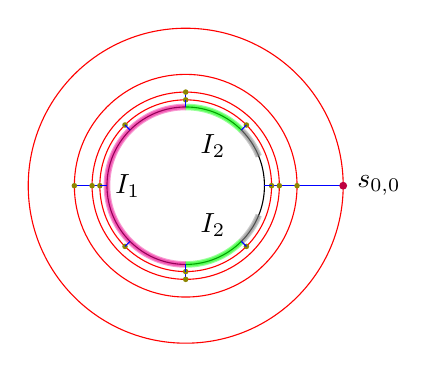
\begin{tikzpicture}
		
		
		\draw (0,0) circle (1);
		\draw[red] (0,0) circle (2);
		\draw[red] (0,0) circle (2^0.5);
		\draw[red] (0,0) circle (2^0.25);
		\draw[red] (0,0) circle (2^0.125);
		
		
		\draw [magenta,-,
			double=magenta,
			double distance=4\pgflinewidth, opacity=0.4,
			] (0,1) arc (90:270:1);
		
		\draw [green,-,
			double=green,
			double distance=4\pgflinewidth, opacity=0.4,
			] (0,1) arc (90:45:1);

		\draw [green,-,
			double=green,
			double distance=4\pgflinewidth, opacity=0.4,
			] (0,-1) arc (270:315:1);

		\draw [gray,-,
			double=gray,
			double distance=4\pgflinewidth, opacity=0.4,
			] (45:1) arc (45:22:1);
		\draw [gray,-,
			double=gray,
			double distance=4\pgflinewidth, opacity=0.4,
			] (-45:1) arc (-45:-22:1);

		
		\draw[blue] (2,0);
		
		\draw[blue] (2,0) --  (1,0);	
		\draw[blue] (-2^0.5,0) -- (-1,0);	
		\draw[blue] (0, 2^0.25) -- (0,1);	
		\draw[blue] (0, -2^0.25) -- (0,-1);	
		
		\fill[olive] (2,0) circle (1pt);
		\fill[olive] (2^0.5,0) circle (1pt);
		\fill[olive] (-2^0.5,0) circle (1pt);
		
		\foreach \angle in {0,90,180,270}
		\fill[olive] (\angle:2^0.25) circle (1pt);
		
		\foreach \angle in {0,45,90,135,180,225,270,315}
		\fill[olive] (\angle:2^0.125) circle (1pt);
		\foreach \angle in {0,45,90,135,180,225,270,315} 		
		\draw[blue] (\angle:2^0.125) -- (\angle:1);
		
		
		\node[circle,inner sep=1pt,label=left:{$I_1$}] at (-0.4,0) {};

		\node[circle,inner sep=1pt,label=right:{$I_2$}] at (0.01,0.5) {};
		\node[circle,inner sep=1pt,label=right:{$I_2$}] at (0.01,-0.5) {};
		
		\node[circle,inner sep=1pt,fill=purple,label=right:{$s_{0,0}$}] at (2,0) {};
		
	\end{tikzpicture}
	
	\caption{First few parts of the departure decomposition $I_m$ of the circle.
	} \label{fig:departure-decomposition}
\end{figure}

